\documentclass{extbook}[14pt]
\usepackage{multicol, enumerate, enumitem, hyperref, color, soul, setspace, parskip, fancyhdr, amssymb, amsthm, amsmath, latexsym, units, mathtools}
\everymath{\displaystyle}
\usepackage[headsep=0.5cm,headheight=0cm, left=1 in,right= 1 in,top= 1 in,bottom= 1 in]{geometry}
\usepackage{dashrule}  % Package to use the command below to create lines between items
\newcommand{\litem}[1]{\item #1

\rule{\textwidth}{0.4pt}}
\pagestyle{fancy}
\lhead{}
\chead{Answer Key for Module11L Version ALL}
\rhead{}
\lfoot{5317-4125}
\cfoot{}
\rfoot{test}
\begin{document}
\textbf{This key should allow you to understand why you choose the option you did (beyond just getting a question right or wrong). \href{https://xronos.clas.ufl.edu/mac1105spring2020/courseDescriptionAndMisc/Exams/LearningFromResults}{More instructions on how to use this key can be found here}.}

\textbf{If you have a suggestion to make the keys better, \href{https://forms.gle/CZkbZmPbC9XALEE88}{please fill out the short survey here}.}

\textit{Note: This key is auto-generated and may contain issues and/or errors. The keys are reviewed after each exam to ensure grading is done accurately. If there are issues (like duplicate options), they are noted in the offline gradebook. The keys are a work-in-progress to give students as many resources to improve as possible.}

\rule{\textwidth}{0.4pt}

\begin{enumerate}\litem{
List 10 numbers you should use to estimate the one-sided limit of the function below as $x$ approaches 2 from the right.
\[ \frac{\frac{2}{x} - 1}{x - 2} \]The solution is \( \{ 2.1000, 2.0100, 2.0010, 2.0001 \} \).\begin{enumerate}[label=\Alph*.]
\textbf{Plausible alternative answers include:}These values would estimate the limit of 2 on the left.
These values would estimate the limit at the point and not a one-sided limit.
If we get $\frac{0}{0}$ or $\frac{\infty}{\infty}$, the value 2 doesn't help us estimate the limit.
If we get $\frac{0}{0}$ or $\frac{\infty}{\infty}$, the value 2 doesn't help us estimate the limit.
This is correct!
\end{enumerate}

\textbf{General Comment:} \textbf{General Comments:} To evaluate a one-sided limit, we want to put numbers close to the limit. We can't use the limit value itself if it results in $\frac{0}{0}$ or $\frac{\infty}{\infty}$
}
\litem{
Evaluate the limit below, if possible.
\[ \lim_{x \rightarrow 7} \frac{\sqrt{9x - 27} - 6}{6x - 42} \]The solution is \( 0.125 \).\begin{enumerate}[label=\Alph*.]
\textbf{Plausible alternative answers include:}You likely tried to use a shortcut to find the limit of a function that only works for when the numerator/denominator are polynomials.
You likely memorized how to solve the similar homework problem and used the same formula here.
* This is the correct option.
You likely believed that since the denominator is equal to 0, the limit is infinity.
If you got a limit that does not match any of the above, please contact the coordinator.
\end{enumerate}

\textbf{General Comment:} \textbf{General comments:} It is difficult to imagine the graph of this function, so you need to test values close to $x = 7$.
}
\litem{
Based on the information below, what can be said about (a.) $f(0)$ and (b.) $f(x)$ when $x$ is close to $0$?

\begin{center}
    \textit{ As $x$ approaches $0$, $f(x)$ approaches $12.547$. }
\end{center}
The solution is \( f(x) \text{ is close to or exactly } 12.547 \text{ when } x \text{ is close to } 0 \).\begin{enumerate}[label=\Alph*.]
\textbf{Plausible alternative answers include:}




\end{enumerate}

\textbf{General Comment:} The limit tells you what happens as the $x$-values approach $0$. It says \textbf{absolutely nothing} about what is happening exactly at $f(0)$!
}
\litem{
For the graph below, find the value(s) $a$ that makes the statement true: $ \displaystyle \lim_{x \rightarrow a} f(x) = 0$.

\begin{center}
    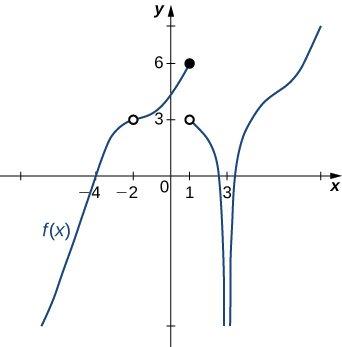
\includegraphics[width=0.5\textwidth]{../Figures/evaluateLimitGraphicallyA.png}
\end{center}


The solution is \( \text{Multiple } a \text{ make the statement true}. \).\begin{enumerate}[label=\Alph*.]
\textbf{Plausible alternative answers include:}




\end{enumerate}

\textbf{General Comment:} \textbf{General Comments:} There can be multiple $a$ values that make the statement true! For the limit, draw a horizontal line and determine if an $x$ value makes the limit exist.
}
\litem{
List 10 numbers you should use to estimate the one-sided limit of the function below as $x$ approaches 6 from the right.
\[ \frac{\frac{6}{x} - 1}{x - 6} \]The solution is \( \{ 6.1000, 6.0100, 6.0010, 6.0001 \} \).\begin{enumerate}[label=\Alph*.]
\textbf{Plausible alternative answers include:}If we get $\frac{0}{0}$ or $\frac{\infty}{\infty}$, the value 6 doesn't help us estimate the limit.
These values would estimate the limit at the point and not a one-sided limit.
If we get $\frac{0}{0}$ or $\frac{\infty}{\infty}$, the value 6 doesn't help us estimate the limit.
This is correct!
These values would estimate the limit of 6 on the left.
\end{enumerate}

\textbf{General Comment:} \textbf{General Comments:} To evaluate a one-sided limit, we want to put numbers close to the limit. We can't use the limit value itself if it results in $\frac{0}{0}$ or $\frac{\infty}{\infty}$
}
\litem{
Based on the information below, what can be said about (a.) $f(2)$ and (b.) $f(x)$ when $x$ is close to $2$?

\begin{center}
    \textit{ $f(x)$ approaches $10.975$ as $x$ approaches $2$. }
\end{center}
The solution is \( f(x) \text{ is close to or exactly } 10.975 \text{ when } x \text{ is close to } 2 \).\begin{enumerate}[label=\Alph*.]
\textbf{Plausible alternative answers include:}




\end{enumerate}

\textbf{General Comment:} The limit tells you what happens as the $x$-values approach $2$. It says \textbf{absolutely nothing} about what is happening exactly at $f(2)$!
}
\litem{
Evaluate the one-sided limit of the function $f(x)$ below, if possible.
\[ \lim_{x \rightarrow 1^-} \frac{1}{(x-1)^8}+6 \]The solution is \( \infty \).\begin{enumerate}[label=\Alph*.]
\textbf{Plausible alternative answers include:}




\end{enumerate}

\textbf{General Comment:} \textbf{General comments:} You should be able to graph the rational function displayed. If not, go back to Module 7 to learn about the general shape of rational functions.
}
\litem{
For the graph below, find the value(s) $a$ that makes the statement true: $ \displaystyle \lim_{x \rightarrow a} f(x) = 0$.

\begin{center}
    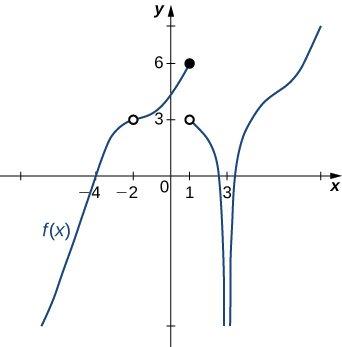
\includegraphics[width=0.5\textwidth]{../Figures/evaluateLimitGraphicallyCopyA.png}
\end{center}


The solution is \( \text{Multiple } a \text{ make the statement true}. \).\begin{enumerate}[label=\Alph*.]
\textbf{Plausible alternative answers include:}




\end{enumerate}

\textbf{General Comment:} \textbf{General Comments:} There can be multiple $a$ values that make the statement true! For the limit, draw a horizontal line and determine if an $x$ value makes the limit exist.
}
\litem{
Evaluate the limit below, if possible.
\[ \lim_{x \rightarrow 7} \frac{\sqrt{4x - 12} - 4}{6x - 42} \]The solution is \( 0.083 \).\begin{enumerate}[label=\Alph*.]
\textbf{Plausible alternative answers include:}You likely learned L'Hospital's Rule in a previous course, but misapplied it here.
You likely memorized how to solve the similar homework problem and used the same formula here.
* This is the correct option.
You likely believed that since the denominator is equal to 0, the limit is infinity.
If you got a limit that does not match any of the above, please contact the coordinator.
\end{enumerate}

\textbf{General Comment:} \textbf{General comments:} It is difficult to imagine the graph of this function, so you need to test values close to $x = 7$.
}
\litem{
Evaluate the one-sided limit of the function $f(x)$ below, if possible.
\[ \lim_{x \rightarrow -6^+} \frac{3}{(x+6)^7}+1 \]The solution is \( \infty \).\begin{enumerate}[label=\Alph*.]
\textbf{Plausible alternative answers include:}




\end{enumerate}

\textbf{General Comment:} \textbf{General comments:} You should be able to graph the rational function displayed. If not, go back to Module 7 to learn about the general shape of rational functions.
}
\litem{
List 10 numbers you should use to estimate the one-sided limit of the function below as $x$ approaches 7 from the right.
\[ \frac{\frac{7}{x} - 1}{x - 7} \]The solution is \( \{ 7.1000, 7.0100, 7.0010, 7.0001 \} \).\begin{enumerate}[label=\Alph*.]
\textbf{Plausible alternative answers include:}These values would estimate the limit at the point and not a one-sided limit.
This is correct!
If we get $\frac{0}{0}$ or $\frac{\infty}{\infty}$, the value 7 doesn't help us estimate the limit.
These values would estimate the limit of 7 on the left.
If we get $\frac{0}{0}$ or $\frac{\infty}{\infty}$, the value 7 doesn't help us estimate the limit.
\end{enumerate}

\textbf{General Comment:} \textbf{General Comments:} To evaluate a one-sided limit, we want to put numbers close to the limit. We can't use the limit value itself if it results in $\frac{0}{0}$ or $\frac{\infty}{\infty}$
}
\litem{
Evaluate the limit below, if possible.
\[ \lim_{x \rightarrow 6} \frac{\sqrt{4x - 8} - 4}{7x - 42} \]The solution is \( \text{None of the above} \).\begin{enumerate}[label=\Alph*.]
\textbf{Plausible alternative answers include:}You likely memorized how to solve the similar homework problem and used the same formula here.
You likely believed that since the denominator is equal to 0, the limit is infinity.
You likely learned L'Hospital's Rule in a previous course, but misapplied it here.
You likely tried to use a shortcut to find the limit of a function that only works for when the numerator/denominator are polynomials.
* This is the correct option as the limit is 0.071.
\end{enumerate}

\textbf{General Comment:} \textbf{General comments:} It is difficult to imagine the graph of this function, so you need to test values close to $x = 6$.
}
\litem{
Based on the information below, what can be said about (a.) $f(7)$ and (b.) $f(x)$ when $x$ is close to $7$?

\begin{center}
    \textit{ $f(x)$ approaches $10.049$ as $x$ approaches $7$. }
\end{center}
The solution is \( f(x) \text{ is close to or exactly } 10.049 \text{ when } x \text{ is close to } 7 \).\begin{enumerate}[label=\Alph*.]
\textbf{Plausible alternative answers include:}




\end{enumerate}

\textbf{General Comment:} The limit tells you what happens as the $x$-values approach $7$. It says \textbf{absolutely nothing} about what is happening exactly at $f(7)$!
}
\litem{
For the graph below, evaluate the limit: $ \displaystyle \lim_{x \rightarrow -4} f(x)$.

\begin{center}
    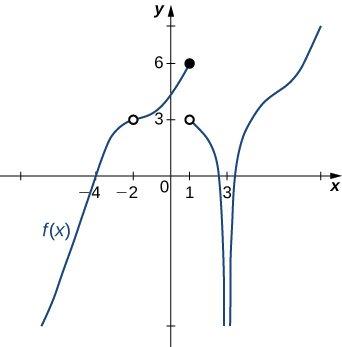
\includegraphics[width=0.5\textwidth]{../Figures/evaluateLimitGraphicallyB.png}
\end{center}


The solution is \( 0 \).\begin{enumerate}[label=\Alph*.]
\textbf{Plausible alternative answers include:}




\end{enumerate}

\textbf{General Comment:} \textbf{General Comments:} Remember that the limit does not exist if the left-hand and right-hand limits do not match.
}
\litem{
List 10 numbers you should use to estimate the one-sided limit of the function below as $x$ approaches 8 from the left.
\[ \frac{\frac{8}{x} - 1}{x - 8} \]The solution is \( \{ 7.9000, 7.9900, 7.9990, 7.9999 \} \).\begin{enumerate}[label=\Alph*.]
\textbf{Plausible alternative answers include:}If we get $\frac{0}{0}$ or $\frac{\infty}{\infty}$, the value 8 doesn't help us estimate the limit.
These values would estimate the limit of 8 on the right.
These values would estimate the limit at the point and not a one-sided limit.
This is correct!
If we get $\frac{0}{0}$ or $\frac{\infty}{\infty}$, the value 8 doesn't help us estimate the limit.
\end{enumerate}

\textbf{General Comment:} \textbf{General Comments:} To evaluate a one-sided limit, we want to put numbers close to the limit. We can't use the limit value itself if it results in $\frac{0}{0}$ or $\frac{\infty}{\infty}$
}
\litem{
Based on the information below, what can be said about (a.) $f(1)$ and (b.) $f(x)$ when $x$ is close to $1$?

\begin{center}
    \textit{ As $x$ approaches $1$, $f(x)$ approaches $\infty$. }
\end{center}
The solution is \( f(x) \text{ is undefined when } x \text{ is close to or exactly } 1. \).\begin{enumerate}[label=\Alph*.]
\textbf{Plausible alternative answers include:}




\end{enumerate}

\textbf{General Comment:} The limit tells you what happens as the $x$-values approach $1$. It says \textbf{absolutely nothing} about what is happening exactly at $f(1)$!
}
\litem{
Evaluate the one-sided limit of the function $f(x)$ below, if possible.
\[ \lim_{x \rightarrow 1^-} \frac{5}{(x+1)^4}+1 \]The solution is \( f(1) \).\begin{enumerate}[label=\Alph*.]
\textbf{Plausible alternative answers include:}




\end{enumerate}

\textbf{General Comment:} \textbf{General comments:} You should be able to graph the rational function displayed. If not, go back to Module 7 to learn about the general shape of rational functions.
}
\litem{
For the graph below, find the value(s) $a$ that makes the statement true: $ \displaystyle \lim_{x \rightarrow a} f(x) = 0$.

\begin{center}
    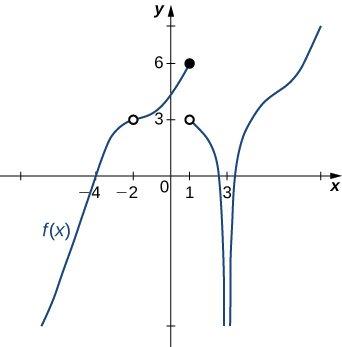
\includegraphics[width=0.5\textwidth]{../Figures/evaluateLimitGraphicallyCopyB.png}
\end{center}


The solution is \( \text{Multiple } a \text{ make the statement true}. \).\begin{enumerate}[label=\Alph*.]
\textbf{Plausible alternative answers include:}




\end{enumerate}

\textbf{General Comment:} \textbf{General Comments:} There can be multiple $a$ values that make the statement true! For the limit, draw a horizontal line and determine if an $x$ value makes the limit exist.
}
\litem{
Evaluate the limit below, if possible.
\[ \lim_{x \rightarrow 5} \frac{\sqrt{4x - 4} - 4}{2x - 10} \]The solution is \( 0.250 \).\begin{enumerate}[label=\Alph*.]
\textbf{Plausible alternative answers include:}You likely learned L'Hospital's Rule in a previous course, but misapplied it here.
* This is the correct option.
You likely believed that since the denominator is equal to 0, the limit is infinity.
You likely memorized how to solve the similar homework problem and used the same formula here.
If you got a limit that does not match any of the above, please contact the coordinator.
\end{enumerate}

\textbf{General Comment:} \textbf{General comments:} It is difficult to imagine the graph of this function, so you need to test values close to $x = 5$.
}
\litem{
Evaluate the one-sided limit of the function $f(x)$ below, if possible.
\[ \lim_{x \rightarrow -7^-} \frac{5}{(x+7)^9}+5 \]The solution is \( -\infty \).\begin{enumerate}[label=\Alph*.]
\textbf{Plausible alternative answers include:}




\end{enumerate}

\textbf{General Comment:} \textbf{General comments:} You should be able to graph the rational function displayed. If not, go back to Module 7 to learn about the general shape of rational functions.
}
\litem{
List 10 numbers you should use to estimate the one-sided limit of the function below as $x$ approaches 4 from the right.
\[ \frac{\frac{4}{x} - 1}{x - 4} \]The solution is \( \{ 4.1000, 4.0100, 4.0010, 4.0001 \} \).\begin{enumerate}[label=\Alph*.]
\textbf{Plausible alternative answers include:}This is correct!
If we get $\frac{0}{0}$ or $\frac{\infty}{\infty}$, the value 4 doesn't help us estimate the limit.
These values would estimate the limit of 4 on the left.
If we get $\frac{0}{0}$ or $\frac{\infty}{\infty}$, the value 4 doesn't help us estimate the limit.
These values would estimate the limit at the point and not a one-sided limit.
\end{enumerate}

\textbf{General Comment:} \textbf{General Comments:} To evaluate a one-sided limit, we want to put numbers close to the limit. We can't use the limit value itself if it results in $\frac{0}{0}$ or $\frac{\infty}{\infty}$
}
\litem{
Evaluate the limit below, if possible.
\[ \lim_{x \rightarrow 8} \frac{\sqrt{7x - 40} - 4}{3x - 24} \]The solution is \( 0.292 \).\begin{enumerate}[label=\Alph*.]
\textbf{Plausible alternative answers include:}* This is the correct option.
You likely memorized how to solve the similar homework problem and used the same formula here.
You likely believed that since the denominator is equal to 0, the limit is infinity.
You likely tried to use a shortcut to find the limit of a function that only works for when the numerator/denominator are polynomials.
If you got a limit that does not match any of the above, please contact the coordinator.
\end{enumerate}

\textbf{General Comment:} \textbf{General comments:} It is difficult to imagine the graph of this function, so you need to test values close to $x = 8$.
}
\litem{
Based on the information below, what can be said about (a.) $f(8)$ and (b.) $f(x)$ when $x$ is close to $8$?

\begin{center}
    \textit{ As $x$ approaches $8$, $f(x)$ approaches $13.449$. }
\end{center}
The solution is \( \text{None of the above are always true.} \).\begin{enumerate}[label=\Alph*.]
\textbf{Plausible alternative answers include:}




\end{enumerate}

\textbf{General Comment:} The limit tells you what happens as the $x$-values approach $8$. It says \textbf{absolutely nothing} about what is happening exactly at $f(8)$!
}
\litem{
For the graph below, find the value(s) $a$ that makes the statement true: $ \displaystyle \lim_{x \rightarrow a} f(x) = -\infty$.

\begin{center}
    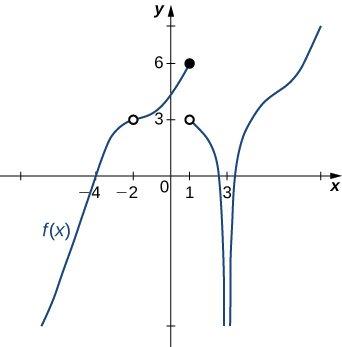
\includegraphics[width=0.5\textwidth]{../Figures/evaluateLimitGraphicallyC.png}
\end{center}


The solution is \( \text{Multiple } a \text{ make the statement true}. \).\begin{enumerate}[label=\Alph*.]
\textbf{Plausible alternative answers include:}




\end{enumerate}

\textbf{General Comment:} \textbf{General Comments:} There can be multiple $a$ values that make the statement true! For the limit, draw a horizontal line and determine if an $x$ value makes the limit exist.
}
\litem{
List 10 numbers you should use to estimate the one-sided limit of the function below as $x$ approaches 10 from the right.
\[ \frac{\frac{10}{x} - 1}{x - 10} \]The solution is \( \{ 10.1000, 10.0100, 10.0010, 10.0001 \} \).\begin{enumerate}[label=\Alph*.]
\textbf{Plausible alternative answers include:}If we get $\frac{0}{0}$ or $\frac{\infty}{\infty}$, the value 10 doesn't help us estimate the limit.
If we get $\frac{0}{0}$ or $\frac{\infty}{\infty}$, the value 10 doesn't help us estimate the limit.
These values would estimate the limit at the point and not a one-sided limit.
This is correct!
These values would estimate the limit of 10 on the left.
\end{enumerate}

\textbf{General Comment:} \textbf{General Comments:} To evaluate a one-sided limit, we want to put numbers close to the limit. We can't use the limit value itself if it results in $\frac{0}{0}$ or $\frac{\infty}{\infty}$
}
\litem{
Based on the information below, what can be said about (a.) $f(3)$ and (b.) $f(x)$ when $x$ is close to $3$?

\begin{center}
    \textit{ $f(x)$ approaches $\infty$ as $x$ approaches $3$. }
\end{center}
The solution is \( f(x) \text{ is undefined when } x \text{ is close to or exactly } 3. \).\begin{enumerate}[label=\Alph*.]
\textbf{Plausible alternative answers include:}




\end{enumerate}

\textbf{General Comment:} The limit tells you what happens as the $x$-values approach $3$. It says \textbf{absolutely nothing} about what is happening exactly at $f(3)$!
}
\litem{
Evaluate the one-sided limit of the function $f(x)$ below, if possible.
\[ \lim_{x \rightarrow -4^-} \frac{4}{(x+4)^7}+4 \]The solution is \( -\infty \).\begin{enumerate}[label=\Alph*.]
\textbf{Plausible alternative answers include:}




\end{enumerate}

\textbf{General Comment:} \textbf{General comments:} You should be able to graph the rational function displayed. If not, go back to Module 7 to learn about the general shape of rational functions.
}
\litem{
For the graph below, find the value(s) $a$ that makes the statement true: $ \displaystyle \lim_{x \rightarrow a} f(x) = 0$.

\begin{center}
    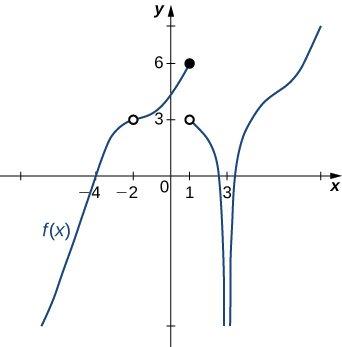
\includegraphics[width=0.5\textwidth]{../Figures/evaluateLimitGraphicallyCopyC.png}
\end{center}


The solution is \( \text{Multiple } a \text{ make the statement true}. \).\begin{enumerate}[label=\Alph*.]
\textbf{Plausible alternative answers include:}




\end{enumerate}

\textbf{General Comment:} \textbf{General Comments:} There can be multiple $a$ values that make the statement true! For the limit, draw a horizontal line and determine if an $x$ value makes the limit exist.
}
\litem{
Evaluate the limit below, if possible.
\[ \lim_{x \rightarrow 4} \frac{\sqrt{8x - 16} - 4}{7x - 28} \]The solution is \( 0.143 \).\begin{enumerate}[label=\Alph*.]
\textbf{Plausible alternative answers include:}You likely believed that since the denominator is equal to 0, the limit is infinity.
You likely learned L'Hospital's Rule in a previous course, but misapplied it here.
You likely memorized how to solve the similar homework problem and used the same formula here.
* This is the correct option.
If you got a limit that does not match any of the above, please contact the coordinator.
\end{enumerate}

\textbf{General Comment:} \textbf{General comments:} It is difficult to imagine the graph of this function, so you need to test values close to $x = 4$.
}
\litem{
Evaluate the one-sided limit of the function $f(x)$ below, if possible.
\[ \lim_{x \rightarrow -4^-} \frac{7}{(x+4)^8}+1 \]The solution is \( \infty \).\begin{enumerate}[label=\Alph*.]
\textbf{Plausible alternative answers include:}




\end{enumerate}

\textbf{General Comment:} \textbf{General comments:} You should be able to graph the rational function displayed. If not, go back to Module 7 to learn about the general shape of rational functions.
}
\end{enumerate}

\end{document}